\documentclass{article}
\usepackage{spconf,amsmath,graphicx,hyperref}


\usepackage{cite}
\usepackage{hyperref}
\usepackage{amsmath,amssymb,amsfonts}
%\usepackage{algorithmic}
\usepackage{graphicx}
\usepackage{textcomp}
\usepackage{multirow}
\usepackage{longtable}
\usepackage{xcolor}
\def\BibTeX{{\rm B\kern-.05em{\sc i\kern-.025em b}\kern-.08em
    T\kern-.1667em\lower.7ex\hbox{E}\kern-.125emX}}

\newcommand{\T}{{\scriptscriptstyle \top}}
\usepackage{algorithm}
\newcommand{\comment}[1]{}
\usepackage{algpseudocode}
\usepackage{multirow}
\usepackage{booktabs}
 \newcommand{\Var}{\mathrm{Var}}
\usepackage{amsthm}
  %  \ninept
    
\begin{document}

\title{Instance-Dependent Conformal Prediction with Temporal Adaptation for Time-Series Forecasting}


\author{\IEEEauthorblockN{Lior Frenkel}
\IEEEauthorblockA{\textit{Bar-Ilan University}\\
Ramat-Gan, Israel}
%email address or ORCID}
\and
\IEEEauthorblockN{ Shlomo E. Chazan}
\IEEEauthorblockA{\textit{Bar-Ilan University}\\
Ramat-Gan, Israel }
%email address or ORCID}
\and
\IEEEauthorblockN{Jacob Goldberger}
\IEEEauthorblockA{\textit{Bar-Ilan University}\\
Ramat-Gan, Israel }
%\\jacob.goldberger@biu.ac.il}
}


\newtheorem{proposition}{Proposition}
% Recommended for tables.




\maketitle

\begin{abstract}
Time-series forecasting requires reliable uncertainty estimates for risk-aware decision making. 
Although conformal prediction provides model-agnostic prediction intervals with finite-sample, distribution-free coverage guarantees under exchangeability, applying it to time-series data is challenging because temporal dependence and nonstationarity generally violate exchangeability.
Existing conformal approaches for time series primarily adapt calibration to temporal distribution changes, while the resulting intervals may not adequately reflect the difficulty of individual forecast instances. We propose a conformal framework that combines two complementary forms of adaptation: instance-level adaptation, obtained by normalizing residuals using model-predicted uncertainty, and temporal adaptation, obtained through a continuously updated conformal calibration window. We instantiate the framework using probabilistic forecasting models, including mixture-of-Gaussian experts, whose predictive variance provides an input-dependent uncertainty estimate.
Experiments on standard multivariate time-series benchmarks show that the proposed approach maintains empirical coverage close to the target level while reducing average prediction-interval width by approximately 40–60\% relative to current methods.


\end{abstract}

\begin{keywords}
time-series, mixture-of-experts, confidence interval, conformal prediction
\end{keywords}


\section{Introduction}

Time-series forecasting plays a central role in many scientific and operational applications, including weather prediction, energy management, transportation, finance, and healthcare. In such settings, an accurate point forecast alone is often insufficient: decision makers must also understand the uncertainty associated with each prediction. For example, in weather forecasting, the consequences of underestimating uncertainty may range from inefficient resource allocation to inadequate preparation for extreme events. Reliable prediction intervals are therefore essential for communicating forecast uncertainty and supporting risk-aware decision making.

Traditional approaches to uncertainty quantification typically rely on parametric assumptions about the forecast errors or on probabilistic models that explicitly estimate the conditional distribution of future observations. However, these assumptions may be difficult to verify and can lead to poorly calibrated uncertainty estimates when the forecasting model is misspecified or when the data distribution changes over time. These limitations are particularly important in modern time-series applications, where flexible machine-learning and deep-learning models can achieve high predictive accuracy but do not naturally provide prediction intervals with reliable statistical coverage.

Conformal Prediction (CP) \cite{vovk2005conformal} provides a model-agnostic framework for converting the output of an arbitrary prediction model into prediction intervals with a user-specified coverage level. Under exchangeability, conformal methods offer finite-sample, distribution-free marginal coverage guarantees without requiring a correct probabilistic model for the data. This combination of flexibility and statistical validity has made conformal prediction an attractive approach to uncertainty quantification in classification and regression tasks. Its application to time-series forecasting, however, is not straightforward because observations collected over time are generally dependent and nonstationary, violating the exchangeability assumption underlying classical conformal guarantees.



Several studies have extended conformal prediction to time-series forecasting, where temporal dependence and distribution shifts violate the exchangeability assumption used by standard conformal methods.  A simple approach is to use a rolling window mechanism where the calibration set is dynamically updated. At every time step, the newest nonconformity score is added and the oldest is removed. This handles nonstationarity by assuming that recent scores are more relevant than old scores. Xu and Xie proposed EnbPI, which constructs sequential prediction intervals using bootstrap ensemble forecasts and a sliding window of recent residuals \cite{xu2021enbpi}. They later introduced SPCI, which models the conditional distribution of future nonconformity scores based on previous scores, allowing the interval width to adapt to temporal changes in forecast uncertainty \cite{xu2023spci}. Gibbs and Candes proposed adaptive conformal inference, which dynamically updates the target miscoverage level and provides long-run coverage control under arbitrary distribution shifts \cite{gibbs2021adaptive}.
 Stankevičiūtė et al. introduced conformal time-series forecasting for recurrent neural networks, calibrating prediction regions across multiple forecast horizons \cite{stankeviciute2021conformal}. Auer et al. proposed HopCPT, which uses modern Hopfield networks to select historical nonconformity scores that are relevant to the current forecasting context \cite{auer2023hopcpt}.
% These methods improve conformal prediction for dependent data through different forms of adaptivity and validity, depending on their assumptions regarding temporal dependence and distribution shift.
 Despite these advances, existing time-series conformal methods primarily adapt to changes in the residual distribution over time. They generally do not exploit model-based, input-dependent uncertainty to adapt interval width to the difficulty of the particular forecast instance. Consequently, temporal adaptation and instance-dependent adaptation have largely been treated separately.

%In this work, we study instance-dependent conformal prediction for time-series forecasting, with particular emphasis on weather data. We consider probabilistic Mixture-of-Expert (MoE) models that provide both a point prediction and an input-dependent estimate of predictive uncertainty. The uncertainty estimate is used to normalize the forecast error, and conformal calibration is then applied to obtain prediction intervals whose widths adapt to the current forecasting conditions. To address temporal nonstationarity, the calibration scores are maintained using a rolling calibration window. The resulting framework combines two complementary forms of adaptivity: instance-level adaptation through the predicted uncertainty and temporal adaptation through continuously updated conformal calibration.  Weather forecasting provides a particularly challenging setting for evaluating this approach because weather observations exhibit strong temporal dependence, seasonality, spatial heterogeneity, heteroscedastic errors, and occasional abrupt changes. Our experiments examine whether instance-dependent scaling can produce narrower and more informative prediction intervals than fixed-width conformal methods while maintaining the desired empirical coverage over time. The proposed framework is model-agnostic and can be applied on top of a broad range of neural time-series forecasting architectures.


In this work, we study instance-dependent conformal prediction for  time-series forecasting. 
We consider probabilistic forecasting models that provide both a point forecast and an input-dependent estimate of predictive uncertainty. The predicted uncertainty is used to normalize the forecast error, producing conformal prediction intervals whose widths adapt to the difficulty of each individual forecast.



Our main contribution is a conformal forecasting framework that combines two complementary forms of adaptation. First, instance-dependent predictive uncertainty is used to normalize nonconformity scores, allowing interval widths to reflect the predicted difficulty of individual forecasts. Second, a rolling calibration window with adaptive conformal inference continuously updates the conformal threshold to account for temporal changes in the residual distribution. The resulting interval width therefore adapts both across instances and over time. We instantiate the framework using Gaussian and mixture-of-Gaussian forecasting models and show that the combined adaptation yields substantially narrower intervals than CQR \cite{cqr2019} while maintaining empirical coverage close to the target level.
\section{Instance- and time-adaptive Conformal Prediction for Time-Series Forecasting}
In this section, we propose a conformal forecasting framework that adapts prediction intervals along two complementary dimensions:
across forecast instances according to their predicted uncertainty, and over time according to changes in the residual distribution.


Applying conformal prediction with the absolute-residual nonconformity score 
$s(x,y)=|y-\hat{y}(x)|$  produces prediction intervals with a common width for all test instances   \cite{kato2023review,zhou2025conformal}.  A fixed-width prediction interval cannot adapt to sample-specific uncertainty and therefore fails to distinguish between cases where the regression prediction is more reliable and those where it is not. A standard way to obtain an instance-dependent calibrated interval is the Conformalized Quantile Regression (CQR) algorithm \cite{cqr2019}.
The CQR algorithm is a calibrated regression method that directly finds a prediction interval without any parametric assumption of the prediction distribution.
It consists of a Quantile Regression (QR) \cite{koenker1978regression} followed by a conformalization step.
Although CQR can adapt to heteroscedasticity, training multiple conditional quantiles using the pinball loss may be sensitive to optimization, quantile crossing, and limited data. In this study, we investigate conformal calibration based on the learned conditional variance of the prediction.
%A recent study showed that applying CP to a network trained with a Gaussian loss function  \cite{Nizhar2025} yields better results than CQR.



%{\bf Mixture of Experts.} We next present a probabilistic MoE framework  that forms the basis of our instance-dependent calibration procedure. Modeling the time-series output by a single Gaussian can be too restrictive. Mixture-of-experts models are particularly suitable for time-series forecasting because temporal data often exhibit heterogeneous and time-varying dynamics. By allowing different experts to specialize in distinct forecasting regimes and combining them according to the current input, an MoE can provide both accurate predictions and instance-dependent uncertainty estimates. This makes it especially appropriate for constructing adaptive conformal prediction intervals whose widths reflect the difficulty of each forecast.
%A MoE network \cite{jacobs1991adaptive} is  defined as follows:
%\begin{equation}\label{eq:moe}
 %   x  \rightarrow  ( w_i(x), \mu_i(x)), \hspace{1cm} i=1,...,k 
%\end{equation} where $x$ denotes the input, $\mu_i$ is the prediction of the $i$-th expert and $w_i$ is the weight the model assigns to that expert's prediction. %The weights satisfy $w_i(x) \ge 0$ and $\sum_i w_i(x)=1$.
%The model's output is then calculated as the weighted sum of these expert predictions:
%%\begin{equation}\label{eq:moe_pred}     \hat{y}(x) = \sum w_i(x)\mu_i(x). \end{equation}
%Typically, an MoE comprises a set of individual expert neural networks (often architecturally identical) that predict the outputs $\mu_i$, along with an additional gating neural module responsible for predicting the expert weights $w_i$. When combining CP with MoE, we can either obtain a fixed-width prediction interval  or we can apply CQR by calibrating an auxiliary QR network.  

{\bf Mixture-of-Gaussian Experts (MoGE).}
We next describe the probabilistic forecasting model used to obtain the input-dependent uncertainty estimate required by the proposed conformal framework.
 Mixture-of-experts models are particularly suitable for time-series forecasting because temporal data often exhibit heterogeneous and time-varying dynamics.
Each expert is associated with an input-dependent variance 
$\sigma^2_i(x)$.
This model assumes that the conditional distribution of the labels $y$ given $x$  is a mixture of Gaussians. 
The MoGE model is defined as follows:  
\begin{equation}\label{eq:mog}
    x  \rightarrow  ( w_i(x), \mu_i(x), \sigma^2_i(x)), \hspace{1cm} i=1,...,k. 
\end{equation}
The MoGE model assumes the following MoG conditional density:
\begin{equation}
f(y|x) = \sum_i w_i(x) N ( y ; \mu_i(x), \sigma_i^2 (x)).
\label{eq:mogdensity}
\end{equation}
The mean $\mu_i(x)$ represents the prediction of the $i$-th expert,  while the variance $\sigma_i^2(x)$ 
represents its estimated conditional variance.
Given  labeled training data $(x_1,y_1),...,(x_n,y_n)$,
the network is trained by minimizing the negative log-likelihood loss function:
\begin{equation}
L(\theta) = -\sum_{t=1}^n \log (\sum_{i=1}^k w_i(x_t) \mathcal{N}(y_t; \mu_i(x_t),\sigma_i^2(x_t))
\label{nll}
\end{equation}
 where $\theta$ denotes the set of network parameters.
At inference time, the model prediction is given by:
 \begin{equation}
 \hat{y}(x) = E ( y|x) = \sum w_i(x)\mu_i(x).
 \end{equation}
The law of total variance implies that:
\begin{equation}
\Var(y|x)  = \sum w_i(x) \sigma_i^2(x) +  \sum w_i(x) (\hat{y}(x)-\mu_i(x))^2.
\label{var-moge}
\end{equation}
The first term of (\ref{var-moge}) can be viewed as the within-expert uncertainty and the second term is the between-expert uncertainty. We denote them by
\begin{align}
\sigma_a^2(x) &= \sum_i w_i(x) \sigma_i^2(x), \label{eq:aleat}\\
\sigma_e^2(x) &= \sum_i w_i(x) (\hat{y}(x)-\mu_i(x))^2, \label{eq:epist}
\end{align}
so that $\Var(y|x)=\sigma_a^2(x)+\sigma_e^2(x)$. The within-expert term is the average of the noise levels reported by the individual experts, weighted by the gating, and the between-expert term measures the disagreement between the expert predictions.


%Mixture-of-Gaussians with Uncertainty-Based Gating (MoGU) is a variant of  MoGE  where the gating weights are directly extracted from experts' variances rather than an additional prediction task in the following way: \begin{equation}    w_i = \frac{ \sigma_i^{-2} }{ \sum_j \sigma_j^{-2}}.     \label{widef}
%\end{equation}
%In other words, each expert is weighted in inverse proportion to its variance (i.e., proportional to its precision).  Further substituting (\ref{widef}) into (\ref{var-moge}) we obtain the variance reported by the MoGU model: \begin{equation} \Var(y|x)  =  \frac{k}{\sum_j \sigma_j^{-2}(x)}  + \sum_i \frac{ \sigma_i^{-2}(x)}{\sum_j \sigma_j^{-2}(x)} (\hat{y}(x)-\mu_i(x))^2.
%\label{var-mogu}
%\end{equation}


{\bf Calibrating a MoGE model. } 
We next propose two variants of an instance-dependent CP procedure for MoGE regression models. The calibration is performed by multiplying the estimated conditional variance of the prediction by a scalar $q^2$ that is learned in a calibration phase. In the case of a single Gaussian this operation is well defined: multiplying the variance by $q^2$ transforms $\mathcal{N}(\mu(x),\sigma^2(x))$ into $\mathcal{N}(\mu(x),(q\sigma(x))^2)$, a distribution with the same mean and a calibrated variance. In the case of a MoG of the form (\ref{eq:mogdensity}), we can still form a CP procedure by calibrating the total variance (\ref{var-moge}).    

Let $(x_1,y_1),...,(x_n,y_n)$ be a calibration set and let $s_i = |y_i-\hat{y}(x_i)|/\sigma(x_i)$ be the corresponding non-conformity scores.  The calibration value $q$ computed by the CP algorithm is the  $\frac{\lceil(n+1)(1-\alpha)\rceil}{n}$ quantile of $s_1,...,s_n$.
 In other words, $q$ is the minimal value for which the true value lies within the prediction interval defined by $q$ for at least a  $(1 - \alpha)$ fraction of the calibration set.
Given a test sample $(x,y)$, define $C_q(x)=[\hat{y}(x)-q\sigma(x),\hat{y}(x)+q\sigma(x)]$.
  The CP theory \cite{vovk2005conformal}  guarantees that, under exchangeability, for  test data $(x,y)$, the value $q$ found by the CP algorithm satisfies:
$1-\alpha \le p(y\in C_q(x))$. 

In the nonstationary time-series setting considered here, exchangeability is generally violated; we therefore use rolling calibration and 
Adaptive Conformal Inference (ACI) \cite{gibbs2021adaptive} to adapt the conformal threshold over time and evaluate coverage empirically.
We maintain a sliding calibration window containing the most recent nonconformity scores, initialized using the validation set. Since the forecasting model is multivariate-input/multivariate-output, calibration is performed independently for each channel and forecast horizon. The calibration window is updated causally as the corresponding test residuals become available. To further account for temporal distribution shifts, we use ACI \cite{gibbs2021adaptive}, which updates the effective miscoverage level according 
to the following recursion, with parameter $\delta$:  
\begin{equation}   \alpha_{t+1} = \alpha_t + \delta\,(\alpha - \mathrm{err}_t),
  \qquad \mathrm{err}_t = \mathbf{1}\{s_t > q_t\},
\end{equation}
Thus, $\sigma(x)$ adapts the interval width to the difficulty of the individual forecast, whereas the time-varying conformal threshold $q$
 adapts it to changes in the residual distribution over time.
 The ACI update provides a distribution-free long-run coverage guarantee: irrespective of the underlying data-generating process, the  time-averaged empiricalmiscoverage frequency converges to the target level $\alpha$ \cite{gibbs2021adaptive}.

Another option to calibrate a MoGE density is to multiply the variance of each Gaussian separately, i.e.\ replacing $\sigma_i(x)$ by $q\sigma_i(x)$.
In this case only the within-expert uncertainty is affected by the calibration procedure and the between-expert uncertainty remains unchanged.
 It can be easily verified that to rescale only the within-expert term and leave the between-expert
term as it is, the non-conformity score becomes:
\begin{equation}
  s_i = \sqrt{\max (0, \frac{(y_i-\hat{y}(x_i))^2 - \sigma_e^2(x_i) }{\sigma_a^2(x_i)})}.
\end{equation}
The calibrated variance term of a test sample is: 
\begin{equation}
\sigma_q^2(x)  = q^2\sigma_a^2(x)+\sigma_e^2(x).
\label{eq:calvar}
\end{equation}

We denote the MoGE calibration based on the total variance by CP-MoG and the calibration procedure based on the within-expert variance by CP-MoG-a. 
%Both options are valid and reasonable extensions of a variance-based calibration of a Gaussian distribution.  We note that CP-MoG corresponds to the MoGE: \[
%\sum_i w_i(x)\,\mathcal{N}\big(y;\,\hat{y}(x)+ q(\mu_i(x)-\hat{y}(x)),(q\sigma_i(x))^2\big),
%\]
%and  CP-MoG-a corresponds to the MoGE:   \[
%\sum_i w_i(x)\,\mathcal{N}\big(y;\,\mu_i(x),(q\sigma_i(x))^2\big).
%\]
In the next section, we empirically compare the performance of the two MoGE calibration methods on the task of time-series prediction.    
The proposed instance-dependent conformal prediction framework with temporal adaptation is summarized in Algorithm~1. 
%Given a confidence level $1-\alpha$, we can next apply CP to the scale $q$ and find a prediction interval around $\hat{y}(x)$ in the form of
%\begin{equation} C_q(x)= [\hat{y}(x)-\sigma_q(x),\hat{y}(x)+\sigma_q(x) ] .
%\label{eq:interval} \end{equation} A labeled example $(x,y)$ is covered by (\ref{eq:interval}) when its squared prediction error does not exceed $q^2\sigma_a^2(x)+\sigma_e^2(x)$, which is a lower bound on the squared scale $q^2$. For each labeled calibration example $(x,y)$ we therefore define the conformal score: \begin{equation} s =  \max\Big(0,\frac{(y-\hat{y}(x))^2-\sigma_e^2(x)}{\sigma_a^2(x)}\Big) ,
%\label{eq:score}
%\end{equation} which subtracts the between-expert term from the squared prediction error and measures the remainder in units of within-expert variance.



%however, multiplying the variance (\ref{var-moge}) by $q^2$ yields
%$$ q^2\Var(y|x)\!=\!\sum_i w_i(x)\big(q\sigma_i(x)\big)^2
%+\sum_i w_i(x)\big(q\hat{y}(x)-q\mu_i(x)\big)^2,
%$$ which is the variance of the MoG
%\[ \sum_i w_i(x)\,\mathcal{N}\big(y;\,q\mu_i(x),(q\sigma_i(x))^2\big). \]
%In other words, scaling the variance of the mixture as a whole also scales the expert means, and the prediction of the calibrated model becomes $q\hat{y}(x)$. Changing the network prediction is not what we expect from a calibration process.


\begin{algorithm}[t]
\caption{Instance-Dependent Conformal Prediction with Temporal Adaptation}
\label{alg:vs_aci}
\begin{algorithmic}[1]
\Require Trained forecasting model providing $\hat{y}(x)$ and $\sigma(x)$;
initial calibration-score set $\mathcal{S}_0$;
target miscoverage level $\alpha$;
ACI step size $\delta$;
calibration-window size $W$.
\State Initialize $\alpha_1 \gets \alpha$
\For{$t=1,2,\ldots$}
    \State \!\!\!\!Obtain the prediction   $\hat{y}(x_t)$ and its uncertainty
        $\sigma(x_t)$.
       \State \!\!\!\!Compute the adaptive conformal quantile: \\
    \hspace{1cm}$
    q_t \gets
    \operatorname{Quantile}_{1-\alpha_t}
    \left(\mathcal{S}_{t-1}\right)
    $.
    \State \!\!\!\!Output:  $C_t(x_t)  \gets [\hat{y}(x_t)\!-\!q_t\sigma(x_t),\hat{y}(x_t)\!+\!q_t\sigma(x_t)]$.
    %$ \left[ \hat{y}(x_t)-q_t\sigma(x_t),\;     \hat{y}(x_t)+q_t\sigma(x_t) \right]$.
    \State \!\!\!\!After $y_t$ becomes available, compute:
    $
    s_t \gets
    \frac{|y_t-\hat{y}(x_t)|}{\sigma(x_t)}
    $.
    \State\!\!\!\!Compute the coverage error:
    $
    \mathrm{err}_t
    \gets
    \mathbf{1}\{s_t>q_t\}.
    $
    \State \!\!\!\!Update the effective miscoverage level using ACI:
    \[
    \alpha_{t+1}
    \gets
    \alpha_t+\delta(\alpha-\mathrm{err}_t)
    \]
    \State \!\!\!\! Update $S_t$ by adding $s_t$ and removing its oldest score.
\EndFor
\end{algorithmic}
\end{algorithm}

\section{Experiments}\label{sec:experiments}


We evaluate the proposed instance- and time-adaptive conformal framework on four multivariate time-series forecasting benchmarks.

\label{sec:experimental_setup}
\textbf{Datasets.}
We evaluate our method on 
%two widely used time series forecasting datasets~\cite{autoformer}: 
%ETTh1 and ETTm1.
four Electricity Transformer Temperature (ETT) datasets (ETTh1, ETTh2, ETTm1, ETTm2)~\cite{informer}.
%Exchange~%\cite{lai2018modeling} and Illness (ILI)\footnote{
%https://gis.cdc.gov/grasp/fluview/fluportaldashboard.html}.



\textbf{Experimental Protocol.} Our experiments follow the standard protocol used in recent time series forecasting literature \cite{Yuqietal-2023-PatchTST,liu2023itransformer, wang2024deep}. For  all datasets, we use a forecast horizon length $h \in \{96,192,336,720\}$. A look-back window of 96 is used for all experiments. 

\textbf{Implementation and Training Details.}
 We used a standard transformer-based state-of-the-art expert model: iTransformer \cite{liu2023itransformer}. It is available from the Time Series Library (TSLib)~\cite{wang2026deep}, with an uncertainty estimation head, as detailed in Section 2.  We trained all models using the Adam optimizer for a maximum of 10 epochs, with early stopping patience set to 3 epochs. The learning rate was set to $\lambda=0.001$. All experiments were conducted on a single NVIDIA A100 80GB GPU. By default, all MoGE configurations utilize three experts, unless otherwise specified.
To handle non-stationarity, we used a sliding calibration window of 1000 scores, initialized from the validation set, and set the ACI parameter to $\delta=0.001$ \cite{gibbs2021adaptive}. Calibration is performed independently for each channel and forecast horizon.
%{\bf Rolling calibration.} Time-series data are neither stationary nor exchangeable, so a fixed calibration set becomes stale as the data distribution drifts. 
%In all our experiments, w



\begin{table}[t]
  \caption{ACI-adapted calibration intervals at a $0.90$ target coverage, ETT datasets, aggregated over 5 training seeds as mean $\pm$ sample standard deviation.  Bold marks the narrowest mean width. }
  \label{tab:ett_aci} 
  \vspace{0.1cm} 
           \scalebox{0.8}{
  \begin{tabular}{l  l  r r}
  \hline
   \textbf{Dataset} &  \textbf{Calibration} & \textbf{Coverage} $\uparrow$ & \textbf{Avg. Width} $\downarrow$ \\

  \hline
  \multirow{5}{*}{ETTm1}   &CP-MoG   & $0.901 \pm 0.000$ & $\mathbf{1.670 \pm 0.030}$ \\*
         & CP-MoG-a & $0.901 \pm 0.001$ & $1.672 \pm 0.029$ \\*
    & CP-G  & $0.901 \pm 0.000$ & $1.704 \pm 0.017$ \\
     & CQR  & $0.899 \pm 0.002$  & $2.774 \pm 0.215$ \\*
     & CQR (retrained) & $0.899 \pm 0.001$ & $1.985 \pm 0.059$ \\
  \hline
  \multirow{5}{*}{ETTm2} &  CP-MoG   & $0.900 \pm 0.000$ &$\mathbf{ 1.538 \pm 0.059}$ \\*
       & CP-MoG-a & $0.900 \pm 0.001$ & $1.540 \pm 0.059$ \\*
      & CP-G  & $0.901 \pm 0.000$ & $1.647 \pm 0.072$ \\*
       & CQR  & $0.890 \pm 0.007$ & $3.943 \pm 0.763$ \\*
     & CQR (retrained)  & $0.897 \pm 0.001$ & $2.209 \pm 0.605$ \\
      \hline
  \multirow{5}{*}{ETTh1} & CP-MoG  & $0.898 \pm 0.001$ & $\mathbf{1.740 \pm 0.004}$ \\*
  & CP-MoG-a & $0.898 \pm 0.001$ & $1.741 \pm 0.004$ \\
     & CP-G  & $0.898 \pm 0.001$ & $1.762 \pm 0.011$ \\*
        & CQR & $0.894 \pm 0.009$ & $3.786 \pm 0.168$ \\*
     & CQR (retrained)  & $0.886 \pm 0.007$ & $2.511 \pm 0.228$ \\
  \hline
  \multirow{5}{*}{ETTh2}  &CP-MoG   & $0.892 \pm 0.001$ & $\mathbf{1.875 \pm 0.036}$ \\*
     & CP-MoG-a & $0.893 \pm 0.001$ & $1.880 \pm 0.035$ \\*
   &  CP-G   & $0.892 \pm 0.001$ & $1.896 \pm 0.066$ \\
 
     & CQR  & $0.886 \pm 0.009$ & $4.460 \pm 0.271$ \\*
     & CQR (retrained) & $0.883 \pm 0.011$ & $3.233 \pm 0.644$ \\
     \hline
   \end{tabular}
   }
\end{table}



\textbf{Evaluation measures.} The standard way to evaluate the performance of confidence-interval estimators on a given test set $(x_1,y_1),...,(x_n,y_n)$ is by computing the degree of coverage and the average length of the prediction intervals.   Smaller average interval widths indicate higher precision.  The length and coverage are formally defined as:
$$ \textrm{length} = \frac{1}{n} \sum_i | C(x_i) |,
\hspace{0.2cm}  \textrm{coverage} = \frac{1}{n} \sum_i 
{\textbf 1}(y_i \in C(x_i))$$
such that $C(x_i)$ is the confidence interval of  $x_i$  and $|C(x_i)|$ is its length.
The best algorithm is the one that reports the minimal average interval length among those that satisfy the coverage requirement. We report CP results across five random initializations (seeds) of the time-series prediction model.   

%\begin{figure}[htbp]
 %   \centering
  %%  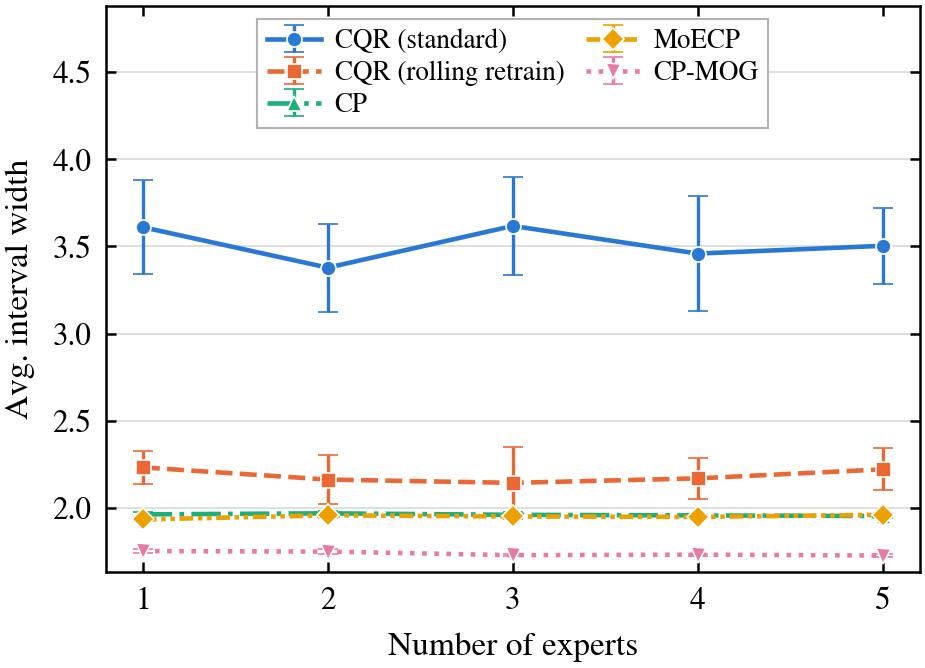
\includegraphics[width=\columnwidth]{avg_width_vs_experts_ETTh1.png}
   % \caption{Average width of the $90\%$ prediction intervals on ETTh1 (iTransformer, horizon $96$) vs.\ the number of experts; mean $\pm 1$ s.d.\ over five seeds.}
    %\label{fig:avg_width_experts_etth1}
%\end{figure}


{\bf Compared methods.} 
We implemented several CP frameworks to generate instance-dependent prediction intervals.
CP-MoG is based on calibrating the total variance and CP-MoG-a is based on calibrating the within-expert part of the variance. 
CP-G is based on calibrating the variance of a single Gaussian model.
We also implemented two variants of  CQR \cite{cqr2019}. CQR requires training a quantile regression network and calibrating its results.
In the first variant (denoted CQR(retrained)), we trained a new QR network for each sliding window and in the second variant, we used a fixed QR network and recalibrated it for each sliding window.


{\bf Results.} Table \ref{tab:ett_aci} summarizes the calibration results, showing that the average interval width (Avg. Width) obtained by
CP-MoG is substantially smaller than that achieved by CQR. The reported empirical coverage values are close to the target level of $90\%$ in almost all cases.
The strong performance obtained even with a single-Gaussian uncertainty model demonstrates that the benefit of the proposed framework is not specific to mixture-of-experts architectures. MoGE provides an additional improvement by offering a richer estimate of predictive uncertainty.
 We observe that even a single-Gaussian model yields considerably better results than CQR. Using multiple experts further improves the results. In the case of MoGE, we did not observe a significant difference between using the total variance and using only the within-expert component. 
 The nearly identical performance of CP-MoG and CP-MoG-a suggests that, for these datasets and prediction models, the within-expert component dominates the predictive variance.
To quantify this, we compute the ratio of the aleatoric to the epistemic variance component, $\mathbb{E}[\sigma_a^2(x)] / \mathbb{E}[\sigma_e^2(x)]$, pooled over all test points and all five seeds: $216$ on ETTh1, $72$ on ETTh2, $163$ on ETTm1, and $189$ on ETTm2. The aleatoric term therefore dominates the total predictive variance by roughly two orders of magnitude on every dataset, which explains why CP-MoG and CP-MoG-a perform nearly identically.
We further assess how informative the total predicted variance $\sigma_a^2(x)+\sigma_e^2(x)$ is about the realized squared error $(y-\hat{y}(x))^2$ via their Pearson correlation, again pooled over all test points and seeds. The correlation is substantially higher on ETTh1 ($r=0.435$) and ETTm1 ($r=0.339$) than on ETTh2 ($r=0.132$) and ETTm2 ($r=0.114$), indicating that the variance head is more informative about instance-level forecast difficulty on ETTh1/ETTm1 than on ETTh2/ETTm2.
   The fixed CQR model generally produces substantially wider intervals and, in the case of ETTm1, also exhibits considerable undercoverage. Retraining the QR model for each window improves its performance, but at the cost of substantially higher computational complexity.
  At comparable coverage, CP-MoG reduces the average interval width by approximately 40–60\% relative to CQR across the four ETT datasets.



\section{Conclusion}
We introduced an instance-dependent conformal prediction framework for multivariate time-series forecasting that combines model-based uncertainty estimation with rolling calibration. Using probabilistic models, the proposed approach scales prediction intervals according to the estimated difficulty of each forecasting instance, while the rolling calibration window helps account for temporal nonstationarity. Experiments on standard time-series benchmarks show that variance-scaled conformal calibration can maintain empirical coverage close to the desired level.
These results demonstrate that instance-dependent uncertainty scaling and temporal conformal adaptation provide complementary forms of adaptivity: the former adjusts interval width to the difficulty of each forecast, while the latter tracks changes in the residual distribution over time. Their combination yields efficient prediction intervals under nonstationary time-series conditions.





\small
\bibliographystyle{IEEEbib}
\bibliography{paper}


\end{document}
